
\documentclass[12pt,journal,compsoc]{IEEEtran}

% Copy package text here:

\usepackage{graphicx}

\begin{document}

\title{Literature Review}
\author{Nicholas Tee}

\date{11/18/2021}

\markboth{ My Name \LaTeX\ Tutorial}%
{Moulds \MakeLowercase{\textit{et al.}}: CMPE185}



\maketitle

%----- The SECTION Environment -------------------------------------------------------------------

% To create a section, simply type the command \section{} with the name of your section name inserted into the curly brackets {}. The section's body text follows underneath the \section{} command. 

\section{Introduction}
The main focus of this paper will be to discuss the current state of research on machine learning and artificial intelligence. It will focus on the applications researchers have used this technology for and how it may affect our quality of life. The paper will discuss three different documents that focus on advancements and applications in computer graphics and computer vision. The first paper will talk about the usage of computer vision technology to detect deepfakes. The second will talk about the effectiveness of our current facial recognition algorithms that are in use today and the flaws that they contain. The final paper will discuss a new method of enhancing resolution in videos.

\section{Counteracitng Deepfakes}
The first paper I want to talk about is “DeepFakesON-Phys: DeepFake Detection based on Heart Rate Estimation” by Javier Hernandez-Ortega, Ruben Tolosana, Julan Fierrez, and Aythami Morales, from the Biometrics and Data Pattern Analytics lab in Universidad Autonoma de Madrid. This paper tackles something that I think is overlooked. Most people are familiar with what a deep fake is; what people overlook is the growing technology steadily improving deep fakes. Although the technology comes with many benefits through its various applications, it can also bear malice. Especially in this time when the internet and media usage is at an all-time high, we are very susceptible to misinformation. The act of spreading fake news can be detrimental in many different ways. For instance, someone could easily use a deep fake to disguise as a government official and misinform the general public about very sensitive or essential topics. An example of this already exists, Jordan Peele used this technology to create a video of him disguised as former US president Barack Obama, the video was made three years ago. \\\\
Attempts to detect deep fakes have already been made. However, they are not that effective and are prone to detecting plenty of false-positive results. The paper challenges the use of physiological features to detect deep fakes. The paper does not go into too much technical detail on how the system works. What is mentioned is that the project uses existing results and tech made purely for the detection of heart rates. The DeepPhys deep learning model trained for heart rate estimation was implemented and modified to detect deep fakes. The final heart rate estimation is not used as a factor, but rather the information that is linked to the prediction of a person’s heart rate is what is used. The system has two main steps when processing the videos. The system will first process the frames into a “Normalized Frame Difference” and a “Normalized Frame” for each frame. Once the frame has been processed, the “Normalized Fram Difference” will be put through the Motion model, designed to detect changes between consecutive frames. At the same time, the “Normalized Frame” is put through the Appearance Model, which analyzes the static information in the frame and determines which frames are the most likely to contain good information on whether or not a deep fake exists in the video. That information is then passed to the Motion model. \\\\
The paper also goes through the multiple tests that the group has done. They first took their system and compared its effectiveness and accuracy with previous studies. They looked at over ten studies and used the same databases that they did. This can be seen through the table that is presented in the table.
\begin{figure}[!h]
  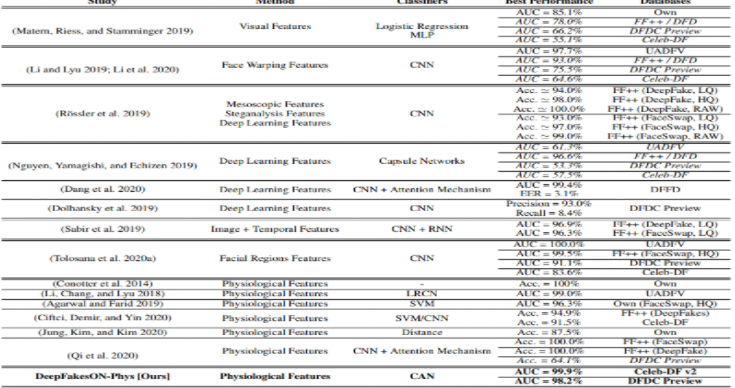
\includegraphics[scale=0.45]{image.png}
  \caption{Figure1: table from paper (Harnandex-Ortega et al)}
  \label{fig:slugman}
\end{figure}
In figure 1, you can see the different researchers, their methods, and their maximum accuracies with specific databases. You can see that all the methods that use physiological features seem to be far more effective than the rest. You can also see that between all the physiological studies, the method proposed in this paper was the most effective. It is difficult to critique their solution since I do not have an in-depth knowledge of how their system functions. However, the one critique that I can give is that I would like to see its effectiveness when using its average accuracy rather than its best performance. I would also like to see its effectiveness with random videos on the internet, rather than a set of databases that have already been used throughout the years.
\newpage
\section{Face Recognition}
The following paper that I read is titled“On the Robustness of Face Recognition Algorithms Against Attacks and Bias” by Richa Singh, Akshay Agarwal, Maneet Singh, Shruti Nagpal, and Mayank Vatsa from IIIT-Delhi. The paper's primary focus is on face recognition technology and the recognition models that are used today. The paper challenges the robustness of said models. The paper talks about how these models, although reliable in some ways, are still susceptible to digital attacks and biases. These attacks refer to alterations made in the image that the model processes. Biases refer to how some models are more effective and accurate with specific population subsets than others. This is an important issue because, when face recognition becomes a more popular method of identification, we need to be sure that the systems in use are as robust as possible. If not, this could lead to identity theft or illegal access to sensitive information. \\\\
The paper goes over several different types of attacks and how they affect the accuracy of face recognition software. These different methods include presentation attacks, which refers to an attack directly at the system, disguise, makeup, and plastic surgery. Initially, I thought that what the paper was covering was somewhat redundant. I thought many of these “attacks” were particular cases that we would not normally encounter in the real world. However, I realized that the paper was trying to show how people may exploit the minor flaws within these recognition models to benefit themselves. Since this is still all relatively new technology, there is still much to learn and improve. Since face recognition is about finding a face despite all the slight variations present in the input image, I think that this paper can give others insight into the flaws of recognition software and use this research to improve our current tech.
\newpage
\section{Image Enhancements}
The last paper that I want to summarize is titled “Low-Resolution Information Also Matters Learning Multi-Resolution Representations for Person Re-Identification” by Guoqing Zhang, Yuhao Chen, Weisi Lin, Arun Chandram, Xuan Jing. This project focuses mainly on a new method of sharpening videos. We know that despite all the advancements in camera technology, most security cameras still suffer from low-resolution images. Thus, much effort has been put into increasing and improving the image quality of the videos. The paper proposes that instead of focusing on improving the image quality soley, we should use the already available information that exists within the low-resolution version of the images.\\\\
A model that takes in both a low and high-resolution image as training data is then used to reconstruct the image. The network in question has different branches. Each branch focuses on a distinct feature of the image. The paper also shows the system's effectiveness relative to previous studies and their methods of increasing resolutions. It is shown that the technique that they proposed seems to be much more effective and accurate. I wanted to talk about this paper as I think that the problem that this solution is challenging is quite essential. If developed to a robust level, I also believe that this technology can be quite helpful in different applications. For instance, this technology can be used in conjunction with the other two papers mentioned in this report to create high-quality images for the training data. It would also mean that we would no longer be limited to high-resolution photos when developing projects such as these three papers.
\newpage
\begin{thebibliography}{1}

\bibitem{IEEEhowto:kopka}
Hernandez-Ortega, Javier, et al. DeepFakesON-Phys: DeepFakes Detection Based on Heart Rate Estimation. Universidad Autonoma De Madrid. 

\bibitem{thing1}
Singh, R., Agarwal, A., Singh, M., Nagpal, S., \& Vatsa, M. (2020). On the Robustness of Face Recognition Algorithms Against Attacks and Bias. Proceedings of the AAAI Conference on Artificial Intelligence, 34(09), 13583-13589. https://doi.org/10.1609/aaai.v34i09.7085

\bibitem{thing2}
Zhang, Guoqing, et al. Low Resolution Information Also Matters ... - Ijcai.org. https://www.ijcai.org/proceedings/2021/0179.pdf. 

\end{thebibliography}


\end{document}
